\documentclass[10pt,twocolumn,letterpaper]{article}
\usepackage[review]{cvpr}
\usepackage{amsmath,amssymb,booktabs,graphicx}
\usepackage{algorithm}
\usepackage[noend]{algpseudocode}
\definecolor{cvprblue}{rgb}{0.21,0.49,0.74}
\usepackage[pagebackref,breaklinks,colorlinks,allcolors=cvprblue]{hyperref}
\def\confName{CVPR}
\def\confYear{2027}
\graphicspath{{figures/}}
\newcommand{\ReachPair}{79.4}
\newcommand{\ReachMark}{23.8}
\newcommand{\ReachImage}{64.2}
\newcommand{\AuditSave}{50.3}
\newcommand{\PCal}{67}
\newcommand{\UCal}{53}
\newcommand{\PTest}{105}
\newcommand{\UTest}{90}
\newcommand{\RoleTest}{69}
\newcommand{\PRank}{62}
\newcommand{\URank}{49}
\newcommand{\NHeads}{283}
\newcommand{\NHeadRows}{302}
\newcommand{\LowerHeads}{280}
\newcommand{\MoreHeads}{251}
\newcommand{\MedianDrop}{6}
\newcommand{\PastBand}{202}
\newcommand{\TopRemoved}{4}
\newcommand{\PairHitsP}{1}
\newcommand{\PairHitsU}{11}
\newcommand{\PairAlertsP}{0}
\newcommand{\PairAlertsU}{8}
\newcommand{\IwahitsP}{3}
\newcommand{\IwahitsU}{6}
\newcommand{\FirstHitsP}{4}
\newcommand{\FirstHitsU}{11}
\newcommand{\PairRank}{55}
\newcommand{\PairDrop}{7}
\newcommand{\PairControlHi}{4}
\newcommand{\PairCutoffP}{1.524}
\newcommand{\PairCutoffU}{0.630}
\newcommand{\PairChange}{17.1}
\newcommand{\PairChangeCI}{[7.5, 27.9]}
\newcommand{\PairRelativeP}{-4.0}
\newcommand{\PairRelativeU}{3.6}
\newcommand{\PairRelativePCI}{[$-7.0$, $-1.4$]}
\newcommand{\PairRelativeUCI}{[$-1.4$, 9.5]}
\newcommand{\ReferenceInteraction}{7.5}
\newcommand{\ReferenceInteractionCI}{[1.7, 14.4]}
\newcommand{\PairPrimary}{3.2}
\newcommand{\IpwPrimary}{7.1}
\newcommand{\PairRobustMedian}{0}
\newcommand{\OriginalLearned}{74}
\newcommand{\OriginalDescriptor}{47}

\algrenewcommand\algorithmicrequire{\textbf{Input:}}
\algrenewcommand\algorithmicensure{\textbf{Output:}}

\title{Auditing Unmarked Nodules in the Patient Alert Tail}
\author{Anonymous}

\begin{document}
\twocolumn[{%
\renewcommand\twocolumn[1][]{#1}%
\maketitle
\vspace{-2.2em}
\begin{center}
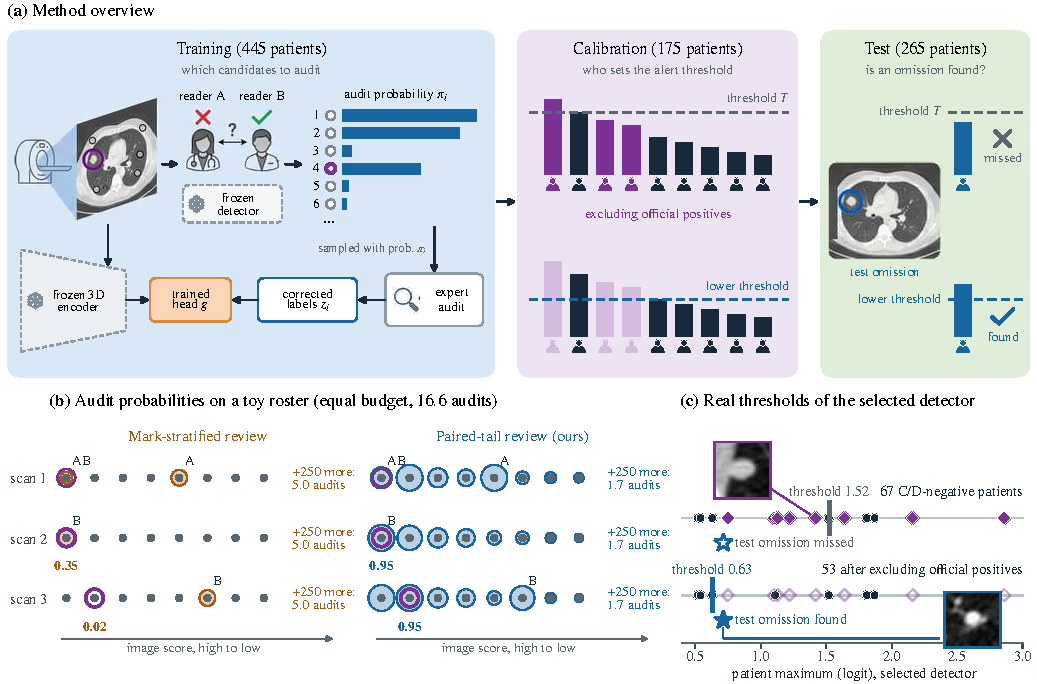
\includegraphics[width=\textwidth]{teaser}
\captionof{figure}{\textbf{The two questions of this paper.} (a)~With the same expected number of re-checks, reviewing candidates in proportion to their reader marks spends most of the budget on the hundreds of unremarkable candidates in every scan, and an unmarked nodule (thick ring) is rarely re-checked. Our paired-tail review favours candidates that rank high in their scan or on which the two weak readers disagree. The discs are computed with the actual allocation rules (Sec.~\ref{sec:audit}) on a toy roster. (b)~The alert cutoff is an upper order statistic of the maximum scores of \emph{negative} calibration patients. Several of the largest maxima (purple) belong to patients with a nodule in the official LUNA16 consensus. Excluding them, with every score unchanged, lowers the cutoff from \PairCutoffP{} to \PairCutoffU{}, and a test omission that was missed is now found. Real values for the selected detector; CT crops are 28\,mm wide.}
\label{fig:teaser}
\end{center}
\vspace{0.8em}
}]

\begin{abstract}
Readers of chest CT sometimes leave a visible lung nodule unmarked. We study two consequences of such omissions. First, if only part of the training data can be re-checked, which candidate locations should be re-checked? Second, when a detector's alert threshold is set on patients labelled negative, how much does the choice of those patients change what the detector appears to find? On LUNA16, a re-check policy that favours candidates near the top of their scan and candidates on which two readers disagree reaches 79 of 92 training omissions in expectation with half the budget. Re-checking in proportion to reader marks reaches 24 with the full budget. More re-checked omissions did not give more detected omissions: our detector found 3.2\% of test omissions versus 7.1\% for the standard baseline, missing our prespecified margin, while finding 3 points more of all nodules. We then keep every detector score fixed and only remove the 14 calibration patients who carry a nodule in the official consensus. The threshold falls for 280 of 283 detectors, and in 202 the fall exceeds the effect of removing 14 patients at random. The selected detector's found omissions rise from 1 to 11 of 42, and its comparison with the baseline changes sign. Who counts as negative deserves the same care as the training labels.
\end{abstract}

\section{Introduction}
\label{sec:intro}

Lung nodule benchmarks are built from radiologists' marks, and radiologists disagree. In the Lung Image Database Consortium (LIDC), four readers marked every scan, yet many lesions were marked by only some of them~\cite{armato2007variability,armato2011}, and the set of ``true'' nodules changes with the readers chosen to define it~\cite{armato2009truth}. Observer studies on LUNA16 found nodules among the detector outputs that the benchmark counted as false positives~\cite{setio2017,jacobs2016cad}. We call a reference nodule that a given reader did not mark an \emph{omission}.

Omissions enter a detection study at two points. During \emph{training}, an unmarked nodule is a negative example unless someone re-checks it, and re-checking (an \emph{audit}) is costly, so only part of the candidates can be audited. During \emph{evaluation}, a detector raises a patient alert when its highest-scoring candidate in a scan exceeds a cutoff. The cutoff is set so that only a fixed fraction $\alpha$ of \emph{negative} calibration patients would alert. A scan with an unmarked nodule can sit in that negative pool, and its high maximum then pushes the cutoff up for every test patient. The two problems meet in the same few high-scoring candidates.

This paper asks one question for each stage (Fig.~\ref{fig:teaser}). (i) Given a fixed audit budget, which training candidates should be audited so that omissions are found? (ii) With all detector scores and all test targets held fixed, how much does the membership of the negative calibration pool move the alert cutoff and the conclusions drawn from it?

For (i), we design \emph{paired-tail} sampling, a probability audit that favours candidates near the top of their own scan or near the alert cutoff, and gives more weight to candidates on which two weak readers disagree. Every candidate keeps a known, positive chance of being audited, so training labels can be corrected without bias. For (ii), we replay the same scores with a negative pool that also excludes patients with a nodule in the official LUNA16 consensus, and compare the change with randomly removing the same number of patients.

Our findings are mixed, and we report them as such. Paired-tail sampling reaches 79.4 of 92 training omissions in expectation at half the audit budget, against 23.8 for the usual mark-stratified design at the full budget (Fig.~\ref{fig:acquisition}). Yet the detector trained on these labels finds fewer test omissions than the mark-stratified baseline at the locked operating point, and fails our prespecified non-inferiority margin (Sec.~\ref{sec:locked}). The reference replay shows why this comparison is fragile. Excluding 14 consensus-positive patients lowers the cutoff by six to seven ranks for the learned detectors, beyond the 95\% range of random removal, and reverses the sign of the method comparison (Sec.~\ref{sec:tail}).

Our contributions are:
\begin{itemize}\itemsep0pt
\item A known-probability audit design for candidate-level re-checking, with exact expected reach of distinct lesions and matched image-only, mark-based and uniform controls.
\item A score-fixed diagnostic that isolates how membership of the negative calibration pool changes a patient-level cutoff, with a size-matched random-removal control and all six reader-pair references.
\item A locked benchmark on LUNA16 that separates three stages, namely which labels are acquired, how well a detector orders candidates within a scan, and where the patient cutoff falls, and reports a negative primary result together with its cause.
\end{itemize}

\section{Related Work}
\label{sec:related}

\paragraph{Reference standards in lung nodule detection.}
LIDC used a two-phase process in which each of four readers first marked blindly and then reviewed the others' marks without forced consensus~\cite{armato2007variability,armato2011}. Agreement remained incomplete, and reader sensitivity varies widely with the panel that defines truth~\cite{armato2009truth}. LUNA16 adopted lesions accepted by at least three of four readers as targets~\cite{setio2017}. Later reading of detector outputs found additional nodules that all four new readers accepted~\cite{jacobs2016cad}. We use this disagreement directly: one reader's marks define omissions, and alternative reference rules define alternative negative pools.

\paragraph{Sparse labels and missed lesions.}
DeepLesion mines clinical bookmarks~\cite{yan2018}. Lesion-Harvester and EnrichedDL add annotations or model outputs to find and correct missed lesions~\cite{cai2021,ma2024}. Multi-reader methods model reader-specific labels or confusion~\cite{tanno2019,wu2024}, and positive--unlabeled learning treats unmarked examples as a mixture~\cite{kiryo2017,bekker2018}. Surveys of label noise in medical imaging cover training-side remedies~\cite{karimi2020noisy}. We instead define omissions against a separate spatial reference and count distinct lesions reached by an audit, including lesions without a high-scoring proposal.

\paragraph{Score-guided acquisition and corrected training.}
Multi-view and volumetric scores support false-positive reduction in CT~\cite{setio2016views,setio2017}, and deep active learning has chosen CT examples by uncertainty~\cite{liu2020active}. Two-phase sampling and active statistical inference use predictions to guide labelling under a budget~\cite{chen2020sampling,zrnic2024active,li2025robust}. Known inclusion probabilities allow unbiased estimation~\cite{horvitz1952}, and augmented inverse-probability weighting with cross-fitting reduces its variance~\cite{robins1994,chernozhukov2018}. Prediction-powered methods are related~\cite{angelopoulos2023ppi,ppssl2025}. We use scan rank and the low-alert cutoff to define where to sample, and test what paired weak marks add at the same budget.

\paragraph{Calibration sets and evaluation labels.}
Conformal and order-statistic cutoffs assume exchangeable calibration scores from the stated population~\cite{angelopoulos2023conformal}, and recent work studies how noisy calibration labels affect them~\cite{einbinder2024label,feldman2026corrupted}. Label errors in test sets can change which model ranks first~\cite{northcutt2021labelerrors}, and validation guidelines stress reference quality and endpoint choice~\cite{maierhein2024metrics}. We measure a related effect for patient alerts: which scans count as negative decides which maxima set the cutoff, even when every candidate score is unchanged.

\ifdefined\ExtendedDraft
  \section{Design and Estimands}
\label{sec:design}

Figure~\ref{fig:map} connects the audit design, image-only fitting, and the patient alert rule. These stages measure target exposure, proposal ordering, and calibrated patient alerts, respectively.

\begin{figure*}[t]
\centering
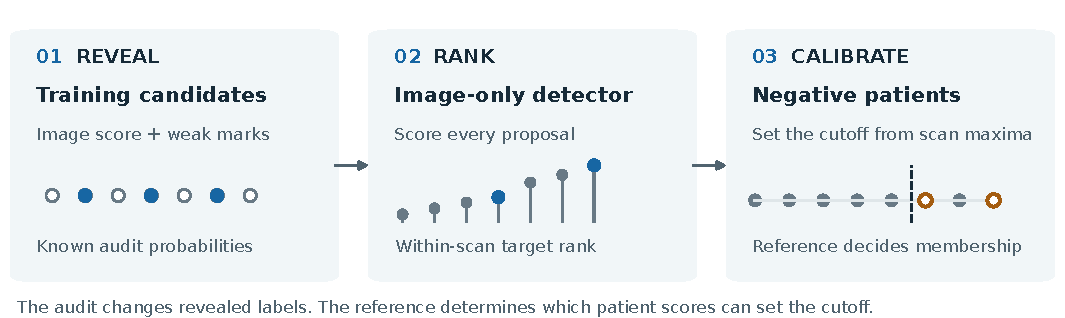
\includegraphics[width=\textwidth]{study_map}
\caption{\textbf{Three stages of omitted-target recovery.} Known-probability audits reveal reference labels on training proposals. The detector scores all proposals using the image alone. Calibration then takes one maximum per reference-negative patient. The reference determines which maxima enter this final step. The symbols illustrate the workflow.}
\label{fig:map}
\end{figure*}

\subsection{Marks, targets, and candidates}

Each patient supplies a fixed roster of candidate locations. Candidate $i$ has image features $X_i$ and weak marks $M_{iA},M_{iB}$, each encoded as marked, assessed and unmarked, or unavailable. A separate pair of reader roles, C and D, defines the original target set. Concordant contours in the released nodule category are linked in physical coordinates before any candidate is scored. The reference label $Y_i$ indicates that the proposal falls in an original target's matching region. An \emph{omission} is an original target without a link to A's contour set. This definition precedes proposal matching. A lesion without any eligible proposal still counts in the omission denominator.

For training, the full original reference is available to the retrospective evaluator. Each audited fit receives only labels selected by its reveal mask. The unobserved proposals still contribute image features and weak marks. On evaluation patients the fitted head takes only image features. A consensus read or an audit is therefore part of supervision or evaluation and supplies no feature to the deployed detector.

\subsection{Allocation and target exposure}

We train a first-read image pilot on development patients and freeze its weights and cutoff $t_0$. For pilot score $s_i$ and descending within-scan rank $r_i$, define
\begin{equation}
 h_i=\max\!\left\{
     \exp[-(r_i-1)/6],\
     \sigma((s_i-t_0+1)/0.7)
 \right\}.
 \label{eq:leverage}
\end{equation}
The rank term retains proposals that can dominate an individual scan even when its absolute scores are low. The second term retains candidates near or above the development cutoff. Their combination avoids relying exclusively on either a global score or a fixed number of proposals per scan.

The image-tail policy uses this score leverage directly. For paired-tail sampling, we also fit an image model of the union of the weak marks in three patient folds. Its out-of-fold predictions and the observed weak-mark count define a bounded working probability $u_i$. For a union-mark probability $p_i$, the three values of $u_i$ are $0.35p_i$, $0.55+0.35p_i$, and $0.92+0.06p_i$ for zero, one, and two marks. Discordant marks receive more weight than agreement when this proxy implies greater uncertainty. The rule requires only information available before the reference label is revealed.

Let $v_i=\max\{u_i(1-u_i),0.006\}$ and $\bar h_i=\max(h_i,0.002)$. Given a candidate budget $B$, we choose probabilities to reduce the separable variance proxy $\sum_i \bar h_i^2 v_i(1/\pi_i-1)$. Differentiation with a budget multiplier gives
\begin{equation}
 \pi_i=\operatorname{clip}(c\bar h_i\sqrt{v_i},\,0.005b,\,0.95),
 \qquad \sum_i\pi_i=B,
 \label{eq:sampling}
\end{equation}
where $b$ is the budget factor and $c$ enforces the expected count. The image-tail policy sets $v_i$ constant. The original mark-stratified policy uses $(0.02,0.35,0.20)b$ for zero, one, and two marks and sets $B$ for all policies at each budget. Uniform sampling uses $B/N$ on $N$ candidates. Each policy draws independent Bernoulli indicators with these probabilities. Corresponding draws share uniforms across policies and share realized masks across the audited training objectives.

A positive audit count can include several proposals for one nodule. We therefore measure unique target exposure. If $\mathcal I_j$ contains the eligible proposal indices for target $j$, its exposure probability is
\begin{equation}
 a_j=1-\prod_{i\in\mathcal I_j}(1-\pi_i).
 \label{eq:exposure}
\end{equation}
The empty product is one. Summing $a_j$ over the fixed training omissions gives the exact expected distinct omissions reached. The same calculation over all candidates in a patient gives the expected number of patients touched. These measures separate spatial yield from candidate and patient workload.

\subsection{Corrected training with audit labels}

Let $R_i$ be the audit indicator and $q_i$ a prediction of the reference label trained outside the proposal's patient fold. We form the target
\begin{equation}
 z_i=q_i+\frac{R_i}{\pi_i}(Y_i-q_i).
 \label{eq:correction}
\end{equation}
A discriminative auxiliary uses the image features, mark indicators, an agreement indicator, and availability, with inverse-probability weights on revealed training labels. An image-only auxiliary uses the same revealed labels and image features. The paired EM auxiliary instead uses a working likelihood that factors the two observed marks conditional on $X_i,Y_i$. All three produce an image-only final head. We also compare direct weighted audit training, supervised fits to each weak read, nonnegative PU with an audited prior, and a fit using all original reference labels.

Conditionally on the pre-audit inputs and the out-of-fold fit, independent inclusion in the held fold gives $\mathbb E_R[z_i]=Y_i$. The logit loss $\ell(z,g)=\log(1+e^g)-zg$ is affine in the label. Thus the corrected risk at any fixed head has the full-reference expectation. This property holds for misspecified auxiliaries and for pre-audit weights. A separate ablation uses loss weight $1+9h_i$ and targets the corresponding weighted reference loss.

Signed targets can have large magnitude. The fitted logits use positive ridge on the coefficients and intercept. Conditional on the fitted auxiliary and $Y_i$, the variance in the label term is $(1-\pi_i)(Y_i-q_i)^2/\pi_i$. The power-tuned control replaces $q_i$ with $\lambda q_i$ and fits a bounded $\lambda$ using an estimate of gradient variance outside the held fold. Equation~\eqref{eq:sampling} targets a surrogate for this uncertainty in the alert tail. Detection after minimizing the random loss and calibrating its scores is an empirical endpoint.

\subsection{Patient alert thresholds}

For a fitted score $g$, let $S_j=\max_{i\in j}g(X_i)$ on patient $j$. Given $n$ reference-negative calibration patients, the strict threshold is
\begin{equation}
 T_\alpha=S_{(k)},\qquad k=\lceil(n+1)(1-\alpha)\rceil,
 \label{eq:threshold}
\end{equation}
where the order statistic is ascending and the threshold is infinite if $k>n$. Any proposal strictly above $T_\alpha$ triggers a patient alert. With distinct exchangeable maxima from the specified negative population, the marginal exceedance probability is $(n+1-k)/(n+1)$. We count a target once if any eligible proposal crosses the threshold. Excess calls to a target count toward FP/scan in the locked benchmark.

Let $P$ denote patients negative by the C/D reference, and let $U$ denote patients negative both by C/D and by the official LUNA16 consensus. The latter corresponds to the union of positive designations. Put $E=P\setminus U$. The maximum-score distribution under $P$ is the mixture of the distributions under $U$ and $E$, with weights given by their representation in $P$. If $E$ contributes disproportionately large maxima, admitting $E$ can raise the relevant upper quantile. This occurs even when the target scores and their within-scan ranks are unchanged.

In a finite pool, membership also changes the order-statistic index. After $m$ removals, the $k'$th remaining score was between the $k'$th and $(k'+m)$th scores in the original sorted pool. Random removal with the same $m$ gives a control for this rank effect. A displacement beyond that control indicates that the excluded patients were systematically placed in the original ranking. This is an empirical property of the model and reference combination.

\section{Benchmark and Analysis Protocol}
\label{sec:benchmark}

\paragraph{Data and geometry.}
We use the official LUNA16 V2 candidate locations and discard the challenge class column \cite{setio2017,luna16v2}. The merged roster contains proposals from CAD systems, some developed on the source LIDC scans. We condition on that roster. Each retained scan has four final LIDC reading sessions. These are unblinded records, and the assigned roles within a scan have access to shared initial marks \cite{armato2011}. A seeded permutation assigns roles A--D. We match C/D contours one-to-one within the greater of 3\,mm and the mean contour radius. Their mean centers and sizes define the original target geometry. The original weak-mark and target matching rules use fixed distance thresholds. The official reference instead requires three of four LIDC readers to agree on a nodule in its inclusion category. The score-fixed analysis uses the official list only to identify additional patients with an official target. Official FROC uses different reference and exclusion rules.

\paragraph{Splits and representations.}
From 888 official series, we exclude one later scan from a repeated TCIA patient and two with other than four reading sessions. The final fit, calibration and test sets contain 445, 175 and 265 distinct patients. The fit uses subsets 0, 1 and 3--5, calibration uses 2 and 6, and test uses 7--9. Prior analyses had inspected regions of the public held-out scans, so the original locked experiment is retrospective. It freezes the heads, seeds, contrasts, and criteria before scoring the designated calibration and test subsets. The 67 original negative calibration patients set rank 62 at nominal $\alpha=0.10$.

The factorial holds the roster fixed across handcrafted and learned image features. The former uses 32 local intensity and multiscale Hessian descriptors \cite{li2003}. The latter uses a 32-dimensional embedding from a 3D CNN on 24\,mm proposal-centered patches. The encoder is trained from scratch on first-role marks from 267 development-fit patients and frozen before the head comparison. The controlled cap retains the largest first-read mark, and its encoder is trained on the capped labels. The full-reference head uses all training labels with the same frozen features and ridge. The supplement gives the network, coordinate matcher, and development gate.

\paragraph{Locked comparisons.}
The original primary endpoint is recall on observed first-reader omissions. Development selected half-budget paired-tail allocation with discriminative augmentation against base-budget mark IPW. The locked efficiency criterion requires a saving in candidate audits, lower confidence limits within five points on both recall endpoints, and comparable alerts and FP/scan. We retain first read, nnPU, and equal-budget uniform, mark, and image-tail controls. The factorial uses a common mark-stratified audit draw. Patient intervals resample test patients jointly across heads and across the six matched audit draws. Audit and negative-calibration resampling characterize separate sources of variability. A calibration-only matched-alert check uses thresholds derived on one negative subset and applied to another to select a comparable operating point.

\paragraph{Score-fixed follow-up.}
After observing the original result and an anchor sensitivity check, we evaluated reference membership for every locked observed-arm fit. Two extra heads reuse the separately trained epoch-16 multi-view checkpoint from the development screen, with the same fitting split and ridge. They use first-read or full-reference supervision and extend the stress test to a second learned architecture. We keep all 276 original test targets and all 42 omissions while comparing cutoffs from $P$ and $U$. Both alert counts in this comparison use the same $U$ test support. We also swap calibration membership across the six unordered pairs of reader roles, with a common test-negative support across all pairs and the official list. These follow-ups share patients with the locked study. The figures and ledgers distinguish the two analyses.

  \section{What the Audits Reveal and the Heads Recover}
\label{sec:locked}

\subsection{Target exposure at a fixed candidate budget}

Paired-tail allocation reaches \ReachPair{} of the 92 observed training omissions in expectation with about 3,950 candidate decisions. Base mark-stratified allocation reaches \ReachMark{} with about 7,900. At the same half budget, mark-stratified and uniform sampling reach 13.0 and 1.4 omissions, respectively, while image-tail sampling reaches \ReachImage{}. Thus most of the increase comes from score information, with a further 15.2 distinct omissions reached by adding the paired evidence at the same budget (Fig.~\ref{fig:acquisition}A). Paired tail reaches 10--17 more omissions than image tail in every matched draw.

The gain extends to double-unmarked omissions, for which no eligible proposal carries either weak mark. The paired and image-tail policies at half budget reach 27.4 and 22.6 of the 35 targets in this group in expectation. Base mark stratification reaches 0.9 (Fig.~\ref{fig:acquisition}B). Since the paired policy cannot use a positive mark on these proposals, this gain reflects the way weak evidence changes the allocation across the entire roster. The image ranking and the probability floor still give double-unmarked locations a route to review.

The realized audit counts agree with the finite-pool expectation. Across the six draws, paired tail at half budget examines an average of 3,940 proposals and reaches 482.7 distinct original targets, including 79.2 omissions. Base mark stratification examines 7,933 proposals and reaches 142.0 distinct targets, including 24.2 omissions. Both policies touch nearly all 445 fit patients. The exposure gain changes how review is distributed \emph{within} patients, an important distinction when opening or reading a scan has a fixed cost.

\subsection{Better features improve proposal ordering}

The 3D representation improves separation between targets and unmatched proposals. In development, the learned full-reference head recovered 38 of 105 targets at nominal 10\% alerts, versus 23 for handcrafted features, with four versus five alerts on 35 negatives. Candidate sensitivity at a descriptive 0.1\% unmatched-candidate FPR rose from 27.7\% to 63.5\%. The initial multi-view checkpoint improved candidate separation and fell short of the development localization gate. The 3D model passed it.

On the locked test set, the 3D full-reference head recovered \OriginalLearned{} of 276 targets versus \OriginalDescriptor{} using descriptors, a paired gain of 9.8 percentage points (95\% interval [3.6, 16.6]). Negative alerts fell from 12 to 2 of 105. The fraction of covered targets ranked above every unmatched proposal in their scan rose from 33.6\% to 67.9\%. The improvement in ranking can be measured without a threshold and agrees with the all-target localization comparison. For observed omissions, the two full-reference heads found two and one of 42, respectively. Image capacity improves overall recovery while the omission subgroup remains difficult at the locked threshold.

\begin{table}[t]
\centering\small
\setlength{\tabcolsep}{3.5pt}
\caption{\textbf{Representation and supervision at the locked anchor.} Each cell reports recovered omissions out of 42, recovered targets out of 276, and alerts out of 105 negative patients. Audited methods share the base mark-stratified draw.}
\label{tab:factorial}
\begin{tabular}{lcc}
\toprule
Supervision & Descriptors & 3D features \\
\midrule
First read & 2 / 39 / 12 & 4 / 81 / 2 \\
Second read & 2 / 37 / 12 & 1 / 76 / 3 \\
nnPU & 2 / 40 / 12 & 3 / 59 / 2 \\
Audit-only IPW & 2 / 57 / 14 & 3 / 70 / 5 \\
Paired EM & 2 / 44 / 12 & 3 / 76 / 3 \\
Image augmentation & 2 / 55 / 12 & 4 / 69 / 5 \\
Discriminative augmentation & 2 / 47 / 11 & 1 / 68 / 4 \\
EM augmentation & 2 / 48 / 10 & 2 / 71 / 6 \\
Power-tuned augmentation & 2 / 48 / 11 & 1 / 69 / 4 \\
Full reference & 2 / 47 / 12 & 1 / 74 / 2 \\
\bottomrule
\end{tabular}

\end{table}

Table~\ref{tab:factorial} reports the supervision factorial, including the simple weak-label, direct audited, and full-reference fits. For learned features, first-read training recovers 81 total targets and four omissions, compared with 74 and one for the full-reference head. These two fits use the same frozen embedding. The full-reference result therefore measures what a linear readout of that embedding does with complete original labels. It is a useful control on supervision and ranking under a shared representation.

\subsection{Omission recovery at the locked threshold}

Across six matched draws, the selected half-budget fit recovers 23.1\% of all targets versus 20.1\% for base-budget mark IPW, a paired gain of 3.0 points [1.3, 4.9]. It uses \AuditSave\% fewer candidate audits. Negative alerts average 2.5\% versus 4.3\%, and FP/scan averages 0.15 versus 0.16. The anchor counts are 69 and 70 all-target detections, so the average effect also reflects variations in which targets the other draws recover.

\begin{table}[t]
\centering\small
\setlength{\tabcolsep}{3.15pt}
\caption{\textbf{Allocation and training under the locked C/D reference.} Entries average the six matched learned-feature draws at nominal $\alpha=0.10$. Recall and alerts are percentages. First read is deterministic given the fit patients and encoder.}
\label{tab:alloc}
\begin{tabular}{lrrrr}
\toprule
Method & Omit.\,$\uparrow$ & All\,$\uparrow$ & Alert & FP/scan\,$\downarrow$ \\
\midrule
First read & \textbf{9.5} & \textbf{29.3} & 1.9 & 0.22 \\
nnPU (base) & 7.1 & 22.6 & 1.9 & 0.20 \\
Mark IPW (base) & 7.1 & 20.1 & 4.3 & 0.16 \\
Mark disc. (half) & 7.5 & 24.5 & 4.4 & 0.16 \\
Uniform disc. (half) & 7.9 & 24.9 & 5.9 & 0.16 \\
Image-tail disc. (half) & 4.8 & 23.2 & 2.4 & 0.17 \\
Paired-tail disc. (half)$^\dagger$ & 3.2 & 23.1 & 2.5 & 0.15 \\
Paired-tail IPW (half) & 4.0 & 24.9 & 2.5 & 0.15 \\
Paired-tail weighted (half) & 2.8 & 26.0 & 2.7 & \textbf{0.14} \\
\bottomrule
\end{tabular}

\end{table}

On the locked primary endpoint, the selected fit averages \PairPrimary\% omission recall versus \IpwPrimary\% for mark IPW, a difference of $-4.0$ points [$-7.0$, $-1.4$]. The lower limit is below the prespecified $-5$-point margin. First-read training recovers 9.5\% of omissions and 29.3\% of all targets with 1.9\% negative alerts and 0.22 FP/scan. At half budget with the same discriminative training, conventional mark, uniform and image-tail allocation reach 7.5\%, 7.9\%, and 4.8\% omission recall, respectively. See Tab.~\ref{tab:alloc} for the full allocation comparison.

\begin{figure*}[t]
\centering
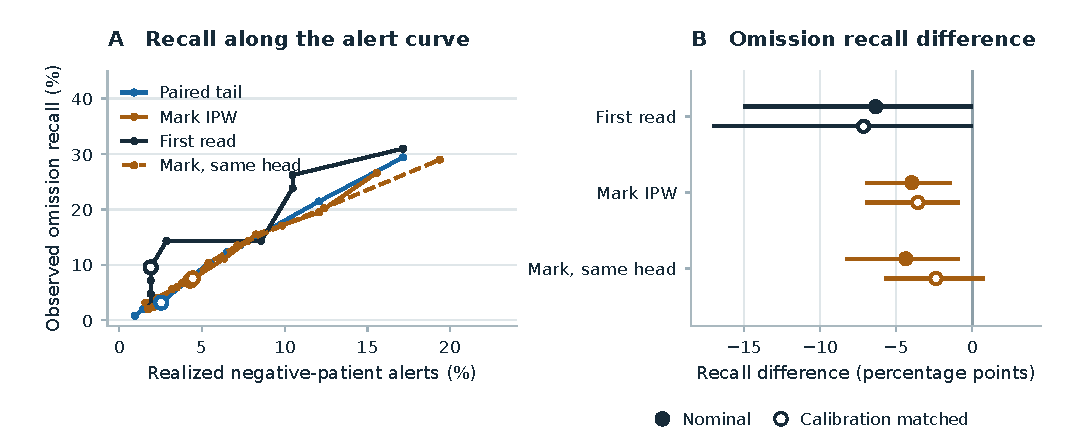
\includegraphics[width=\textwidth]{locked_performance}
\caption{\textbf{Locked localization and paired effects.} (A) Each point uses a calibration-derived cutoff. Open markers denote nominal $\alpha=0.10$. Axes show mean realized test alerts and mean observed omission recall. (B) The selected half-budget fit minus each baseline, with patient-clustered 95\% intervals over the same matched fits. The open points use the calibration-only matched-alert check, whose realized test burdens can still differ.}
\label{fig:locked}
\end{figure*}

The full low-alert curves show a transition from few recovered omissions to much higher recall as the calibration rule admits more alerts (Fig.~\ref{fig:locked}A). Under the calibration-only matched-alert rule, paired-tail omission recall remains 3.6 points lower than IPW [$-7.0$, $-0.9$], and the overall gain shrinks to 0.3 points. The test-patient alert fractions under this rule are 1.7\% and 2.9\%. This check supports the direction of the primary comparison without equating the realized test burdens.

The first-read score, IPW, and the common discriminative head also help locate the effect of the auxiliary. Under the base mark allocation, discriminative and EM augmentation have the same mean omission recall across their three shared draws, and discriminative augmentation shows no clear improvement over image-only augmentation. Power tuning preserves omission counts under the base mark policy. With the selected allocation, tail weighting improves all-target recall by 2.9 points [1.0, 4.8] and changes omission recall by $-0.4$ [$-1.9$, 1.0]. The controlled bookmark cap produces a different pattern. Learned EM augmentation recovers 37 of 151 cap omissions at the anchor versus 25 for first read, with five and four negative alerts respectively. Across its three repeats, EM augmentation recovers 29--37 and audit-only IPW recovers 32--34. The cap tests an imposed size-selection mechanism, with a separately trained encoder and the same physical roster.

\subsection{Locating the missed detections}

All 42 observed omissions have an eligible proposal. At the selected anchor, 16 targets have a candidate ahead of every unmatched proposal in the same scan, and only one crosses the calibrated cutoff. Of the 41 misses, 26 are outranked by an unmatched candidate. The other 15 win that within-scan comparison but remain below threshold. The median rank relative to unmatched proposals is two and the median margin to the cutoff is $-2.22$ logit units. This distinguishes missing localization coverage, which does not occur for this subgroup, from ranking and operating-point losses.

Disputed structures offer a clue about the latter. Only 74 of 45,541 proposals on original negative calibration scans lie near an isolated C or D contour, yet all three sampled maxima near the cutoff have that flag. So do both maxima that trigger an alert on an original negative test scan. In the locked mask sensitivity, masking those candidates at the original cutoff removes both negative alerts and preserves the one recovered omission. Recalibration after masking gives 12 of 42 recovered omissions and five alerts among the 105 original negatives. This intervention changes proposal eligibility. To isolate patient membership, the next analysis keeps the entire roster and scores intact.

  \section{Which Patients Set the Cutoff?}
\label{sec:tail}

\subsection{Changing membership while holding scores fixed}

We compare the original $P$ calibration set with $U$, which excludes any $P$-negative scan containing an official LUNA16 consensus nodule. In calibration this reassigns 14 of 67 original negatives, two from subset 2 and 12 from subset 6. In test it reassigns 15 of 105. Both thresholds are evaluated on the 90 patients negative by both rules. All original test targets remain eligible under both thresholds, including those on reassigned patients. The candidate predictions, target geometry, and omission denominator stay the same. This isolates the effect of changing calibration membership on target calls. It also separates that effect from changes in which patients contribute to the test alert denominator.

\begin{figure*}[t]
\centering
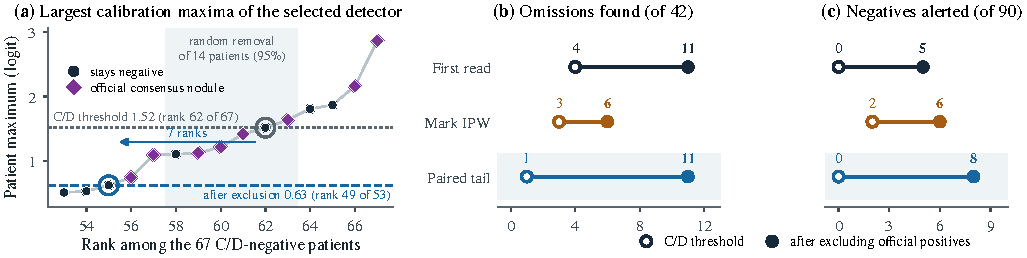
\includegraphics[width=\textwidth]{reference_tail}
\caption{\textbf{A few high maxima move the cutoff while scores stay fixed.} (A) Ordered maxima from the selected anchor among the original negative calibration patients. Diamonds denote patients with an official consensus target. Rings mark the original cutoff and the cutoff after exclusion, both placed on the original rank axis. (B) Original omitted-target calls at the two cutoffs. (C) Alerts on the same 90 common-negative test patients. Both cutoffs use nominal $\alpha=0.10$.}
\label{fig:tail}
\end{figure*}

Figure~\ref{fig:tail}A shows what moves the selected anchor. Three of the six largest maxima are on patients with an official consensus target, and all three maxima spatially match such a target. The C/D cutoff is rank \PRank{} of \PCal{} and has logit \PairCutoffP. The $U$ cutoff is rank \URank{} of \UCal{}. Its original position was \PairRank{}, and its logit is \PairCutoffU. The smaller calibration set therefore selects a score \PairDrop{} ranks below the original threshold. The positions around the threshold matter more than the proportion of all proposals flagged as disputed.

The same selected scores now recover \PairHitsU{} of 42 omissions, compared with \PairHitsP{} before the membership change. Of the ten additional recoveries, five already ranked ahead of every unmatched candidate on their scan. The other five can cross the lower threshold even while another proposal ranks higher. On the same \UTest{} negative test patients, alerts change from \PairAlertsP{} to \PairAlertsU{}. Before the reclassification, the two original negative test alerts were on scans with an official consensus nodule at the flagged location. Their maxima leave the alert denominator, but all of their scores remain in the analysis.

\subsection{How much movement comes from sample size?}

We remove the same number of calibration patients as $U$ does within each original subset, drawing uniformly from the corresponding $P$ negatives. This control retains 53 patients in each of 8,192 paired draws, so the threshold always uses the same smaller-sample rank as $U$. We compare the location of that score on the original rank axis. For the selected anchor the median random displacement is \PairRobustMedian{} ranks, and the upper end of the central 95\% random-removal band is \PairControlHi. The actual seven-rank move is larger (Fig.~\ref{fig:robust}A). The control accounts for the asymmetric deletions from subsets 2 and 6.

The direction holds across model fits. Of the \NHeads{} distinct score vectors from \NHeadRows{} fits, \LowerHeads{} have a lower cutoff with $U$, and the median shift is \MedianDrop{} ranks. The median number of excluded patients among the original six largest maxima is \TopRemoved. For \PastBand{} score vectors the actual displacement exceeds the upper end of the size-matched removal band. The counts describe heads and audit draws evaluated on shared patients.

The capacity of the scorer still matters after calibration moves. At the anchor, both handcrafted fits retain two omission detections even though their cutoffs fall. The multi-view first-read head moves from four to 11 omissions, and its full-reference head moves from three to 11. The corresponding 3D fits move from four to 11 and one to ten. The two learned representations put more omitted targets in the score interval reached by the revised threshold. Table~\ref{tab:reference} records the paired alert counts, which change along with recovery.

\begin{table}[t]
\centering\small
\setlength{\tabcolsep}{3pt}
\caption{\textbf{Fixed-score comparison from original to augmented negative membership.} Each entry gives the result under the $P$ cutoff followed by the result under the $U$ cutoff. The 42 omitted targets, 276 total targets, and 90 common-negative test patients are identical across both cutoffs. Rank drop uses positions in the original calibration pool. Multi-view heads extend the retrospective stress test.}
\label{tab:reference}
\begin{tabular}{lrrrr}
\toprule
Scorer / training & Omit. & All & Alert & Drop \\
\midrule
Descriptors / first & 2 $\to$ 2 & 39 $\to$ 55 & 7 $\to$ 12 & 2 \\
Descriptors / full ref. & 2 $\to$ 2 & 47 $\to$ 57 & 7 $\to$ 10 & 2 \\
Multi-view / first & 4 $\to$ 11 & 66 $\to$ 125 & 1 $\to$ 7 & 6 \\
Multi-view / full ref. & 3 $\to$ 11 & 69 $\to$ 142 & 1 $\to$ 9 & 7 \\
3D / first & 4 $\to$ 11 & 81 $\to$ 133 & 0 $\to$ 5 & 6 \\
3D / full ref. & 1 $\to$ 10 & 74 $\to$ 140 & 0 $\to$ 8 & 7 \\
3D / mark IPW & 3 $\to$ 6 & 70 $\to$ 91 & 2 $\to$ 6 & 6 \\
3D / paired tail & 1 $\to$ 11 & 69 $\to$ 138 & 0 $\to$ 8 & 7 \\
\bottomrule
\end{tabular}

\end{table}

\begin{figure*}[t]
\centering
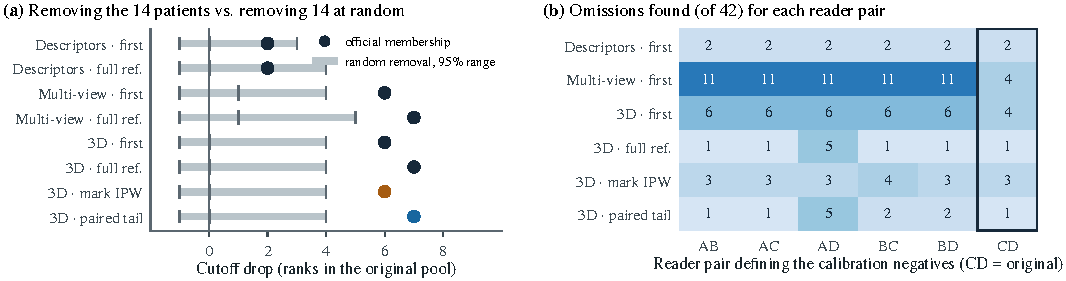
\includegraphics[width=\textwidth]{robustness}
\caption{\textbf{Sensitivity across features, supervision, and reader assignments.} (A) Points show each anchor head's cutoff rank drop under official-consensus augmentation. Gray spans show the central 95\% of the subset-matched random deletion distribution and ticks show its median. (B) Numbers are omitted targets recovered out of the same 42 as calibration varies over all six possible pairs of reader roles. The box identifies C/D, the original assignment.}
\label{fig:robust}
\end{figure*}

\begin{figure*}[t]
\centering
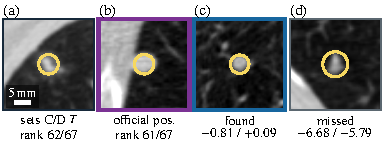
\includegraphics[width=.98\textwidth]{ct_evidence}
\caption{\textbf{The same scored structures can play different roles in calibration and testing.} (A) The candidate at the original calibration cutoff, near an isolated C/D contour. (B) A nearby-ranked maximum that matches an official consensus nodule, on a patient excluded from the augmented negative pool. (C) An original omission newly called at the lower cutoff, with no score change. (D) A covered omission that remains below both cutoffs and has a higher-scoring unmatched distractor. Calibration panels center on the maximum proposal. Test panels center on the original target and give best matched logit minus the original and augmented cutoffs.}
\label{fig:ct}
\end{figure*}

\subsection{Does the choice of reference change the comparison?}

At the original cutoffs the selected paired-tail head recovers \PairHitsP{} anchor omissions against \IwahitsP{} for mark IPW. At the augmented cutoffs those counts are \PairHitsU{} and \IwahitsU{}. On the common-negative patients, their augmented alert counts are eight and six. First read recovers 11 omissions with five alerts. Common test support makes both the change in recall ordering and the accompanying difference in alert burden visible.

Across the six audit fits, paired tail gains \PairChange{} points \PairChangeCI{} in omission recall when changing only the calibration reference. Its mean difference from mark IPW moves from \PairRelativeP{} points \PairRelativePCI{} to $+\PairRelativeU$ points \PairRelativeUCI{}, at the same nominal calibration level. This is a \ReferenceInteraction{}-point shift in the comparison \ReferenceInteractionCI{}. Common-negative alert means under $U$ are 7.2\% for paired tail, 6.1\% for IPW and 5.6\% for first read. The uncertainty intervals resample the test patients jointly and condition on both calibrated sets of scores. The paired shift quantifies the leverage of the negative reference on the method comparison. The C/D result reports the prespecified endpoint under the original reference.

Changing which reader pair defines a negative scan supplies a second stress test without adding any records. For the selected anchor the six pairs give between one and five recovered omissions, with zero to one alerts among the 69 test patients negative under every pair and the official definition. Other learned heads also vary across pairs (Fig.~\ref{fig:robust}B). Different pairs admit different high-scoring patients. Augmenting C/D with the released consensus gives the larger shift and can remove a candidate's entire scan from the negative tail.
\subsection{What the reference checks say about the image}

Figure~\ref{fig:ct} shows why a cutoff-focused examination needs both scores and locations. A large maximum can come from a candidate with documented reader disagreement. Its influence on the cutoff depends on whether the patient remains eligible, even if a separate reader labels the same location positive. Conversely, for a test omission the same nodule can change from a miss to a call solely because a different set of patients calibrated the threshold. A miss can also persist after the shift when an unmatched candidate scores higher and the target remains below both cutoffs. Counts alone merge these cases. Proposal matches, within-scan ranks, and threshold margins let us distinguish them without attributing every miss to a single cause.

  \section{Discussion}

\paragraph{Where paired evidence adds labels.}
Paired-tail sampling reaches more distinct omitted nodules than score-only sampling at the same budget. Its extra reach among targets with no weak marks shows the value of redistributing the review budget across the candidate roster. The within-scan rank and absolute score keep these locations eligible for audit.

\paragraph{What a low-alert evaluation should expose.}
For studies that calibrate a score on reference-negative patients, the patient membership rule deserves the same attention as the spatial matching rule. A useful sensitivity analysis holds candidate scores and target identities fixed, reports the calibration rank and the reference status of the maxima near it, then applies each cutoff to common test support. Size-matched deletions help separate a reference effect from a smaller calibration set. A complementary clinical study would independently adjudicate those maxima and prespecified controls under a declared target scope before repeating the comparison on new patients. In this study both reference rules come from the same four LIDC records. The score-fixed analysis establishes the effect of using those rules on these patients, while independent readings would address whether the excluded cases belong to the intended deployment reference.

\paragraph{Workload and interpretation.}
The observed audit saving is a saving in candidate decisions. The selected and conventional policies touch almost every fit patient, so a scan-opening or navigation cost would reduce proportional time savings. Their mark-based designs also use existing second-reader information. With a different workflow, acquiring that read, running the pilot, choosing an intervention, and evaluating the intervention all contribute to total cost. Those costs and review times were unmeasured. The evidence supports the spatial acquisition gain and the evaluation sensitivity, with the effectiveness of intervention choices at comparable total cost still open.

\paragraph{Limits of the design.}
The learned backbone was trained on first-read marks and frozen before audit-corrected fitting. End-to-end training from revealed labels could alter the ranking stage. The roster is shared across models and inherits LUNA16 candidate provenance. The public CTs had earlier cohort exposure, and the reference checks are retrospective on the same patients. The controlled bookmark cap changes the marking policy and should be interpreted within that intervention. The patient-resampling intervals address variation in the tested population with the fitted scores held fixed.

The study reused public de-identified images and released annotations. It involved no interaction with participants, new data collection, or consent for this secondary analysis. No new ethics review was conducted for this secondary use.

\section{Conclusion}

Paired-tail probability sampling reaches more omitted training nodules at the same candidate budget than sampling by image rank alone. Changing the negative calibration pool moves the cutoff across feature families and changes how detectors compare on the same targets. For low-alert detection studies, these two measurements identify which labels a budgeted audit can reveal and which calibration patients determine when a scored proposal becomes an alert.

\else
  \section{Tail-Guided Auditing and Calibration}
\label{sec:methods}

\subsection{Spatial marks and the CT benchmark}

Each patient has a fixed candidate roster. Proposal $i$ has image features $X_i$ and weak marks from roles A and B, each recorded as marked, assessed and unmarked, or unavailable. The original reference pairs spatially concordant nodule contours from roles C and D. A proposal label $Y_i=1$ means it matches a target under the original geometric rule. An \emph{omission} is an original target with no link to A's marks. This definition precedes scoring and includes targets without an eligible proposal.

We use official LUNA16 V2 coordinates and discard the provided candidate class \cite{setio2017,luna16v2}. The roster merges CAD outputs, including components developed on the LIDC source data. We assign roles by a seeded per-scan permutation of the four final LIDC reading sessions. They are unblinded records with shared initial marks \cite{armato2011}. The original target geometry is the mean center and diameter of paired C/D contours, linked one-to-one within the greater of 3\,mm and the mean contour radius. The supplement specifies the matcher and the complete cohort. The final fit, calibration and test sets contain 445, 175 and 265 distinct patients, with 92 observed training omissions and 42 test omissions. We use official subsets 0, 1 and 3--5 for fitting, 2 and 6 for calibration, and 7--9 for testing.

\subsection{A probability audit for the score tail}

We freeze a development-only first-read image score $s_i$ and its low-alert cutoff $t_0$. For within-scan rank $r_i$ in descending score order, let
\begin{equation}
 h_i=\max\!\left\{\exp[-(r_i-1)/6],\
                    \sigma((s_i-t_0+1)/0.7)\right\}.
 \label{eq:leverage}
\end{equation}
The first term covers proposals that dominate their own scan. The second favors proposals near or above the common cutoff. Image-tail sampling uses $h_i$ alone. Paired tail also estimates the union of the weak marks out of fold using an image model. For its prediction $p_i$ and zero, one or two observed marks, the working probability $u_i$ is $0.35p_i$, $0.55+0.35p_i$, or $0.92+0.06p_i$, respectively. The resulting variance proxy $v_i=\max\{u_i(1-u_i),0.006\}$ gives extra weight to informative disagreements.

Given budget $B$, the design minimizes the surrogate $\sum_i \bar h_i^2v_i(1/\pi_i-1)$ with $\bar h_i=\max(h_i,0.002)$ under a sum constraint and box bounds. The solution is
\begin{equation}
 \pi_i=\operatorname{clip}(c\bar h_i\sqrt{v_i},\,0.005b,\,0.95),
 \qquad \sum_i\pi_i=B.
 \label{eq:allocation}
\end{equation}
Here $b$ is the budget factor and $c$ sets the expected number of candidate decisions. Image tail uses constant $v_i$. Mark stratification uses $(0.02,0.35,0.20)b$ for zero, one and two marks and sets the expected budget for every policy. Uniform selection uses $B/N$ for $N$ candidates. Inclusion is Bernoulli with known positive probabilities. Audit policies share random uniforms, and every training objective within a policy shares the same revealed labels.

For a target $j$ with eligible proposal indices $\mathcal I_j$, the exact chance of exposure is
\begin{equation}
 a_j=1-\prod_{i\in\mathcal I_j}(1-\pi_i).
 \label{eq:reach}
\end{equation}
The empty product is one. Summing over omissions counts distinct reached targets in expectation and separates acquisition from duplicate candidate decisions.

\subsection{Image-only training}

The fixed-roster factorial uses either 32 handcrafted intensity and Hessian descriptors \cite{li2003} or a 32-dimensional embedding from a 3D CNN on 24\,mm candidate patches. The encoder is trained on first-role marks from 267 development patients and frozen. All learned heads in the observed arm share the same embedding. A controlled bookmark arm retains A's largest contour and uses its own first-role encoder. Every deployed head takes image features alone.

Let $R_i$ indicate an audit and let $q_i$ be a reference prediction trained outside the patient's fold. The discriminative auxiliary uses the image embedding and weak-mark indicators, including agreement and availability. The final ridge logit is fit with label
\begin{equation}
 z_i=q_i+\frac{R_i}{\pi_i}(Y_i-q_i).
 \label{eq:augmentation}
\end{equation}
Conditional on the pre-audit inputs and the out-of-fold fit, $\mathbb E_R[z_i]=Y_i$. Logistic loss is affine in its target, so the fixed-head risk has the reference expectation. The signed residual variance is $(1-\pi_i)(Y_i-q_i)^2/\pi_i$. The supplement gives image-only and EM auxiliaries, power tuning, and the weighted-loss ablation. The factorial also includes first- and second-read fitting, nonnegative PU with an audited prior, direct inverse-probability-weighted (IPW) fitting, and a full-reference head.

\subsection{Patient alerts and reference membership}

A patient score is the maximum candidate logit $S_j$. For $n$ reference-negative calibration patients, use the ascending order statistic
\begin{equation}
 T_\alpha=S_{(k)},\qquad k=\lceil(n+1)(1-\alpha)\rceil ,
 \label{eq:cutoff}
\end{equation}
with an infinite cutoff if $k>n$. A proposal alerts on strict exceedance. With distinct exchangeable maxima from the stated negative population, exceedance probability is $(n+1-k)/(n+1)$ \cite{angelopoulos2023conformal}. A target is recovered if any of its proposals exceeds the cutoff. Duplicate alerts count toward FP/scan.

We report two analyses. The locked retrospective comparison uses the original C/D reference and nominal $\alpha=0.10$. Development selected half-budget paired-tail discriminative augmentation against full-budget mark IPW. The original primary endpoint is recall on observed omissions, with a five-point noninferiority margin and prespecified alert and FP/scan limits for the efficiency comparison. Intervals resample test patients jointly across six matched audit draws. The supplement separates audit variation from calibration variation and reports the calibration-only matched-alert check. Earlier work inspected regions of the public evaluation scans. This study froze the weights, endpoints and contrasts before revision scoring on the designated calibration and test subsets.

The score-fixed follow-up changes only which patients qualify as negative. Let $P$ be the C/D negatives and let $U$ be the patients negative under both C/D and the official LUNA16 reference, which requires agreement from at least three of four readers \cite{setio2017}. The $P$ score distribution mixes maxima from $U$ and from $P\setminus U$. Large maxima in the latter group can raise the upper quantile. We preserve all candidate scores and all original test targets, and evaluate both cutoffs on the same $U$-negative test patients. Thus the threshold effect on recovery is isolated from both score changes and changes to the target denominator.

We use 8,192 shared random deletions within calibration subsets, matching the number of exclusions in each subset. With $m$ removals the $k'$th remaining score originally lay between ranks $k'$ and $k'+m$. The random-deletion distribution measures the rank shift expected from the smaller pool. We also rebuild calibration pools for every pair of reader roles, preserving the test target list and using patients negative by every pair and the official reference for the common alert denominator. These follow-ups extend an initial anchor check on the same public cohort.

  \section{Experiments}
\label{sec:yield}

\subsection{Experimental setup}
\label{sec:setup}

\paragraph{Dataset.}
We use the 888 scans of LUNA16 with the V2 candidate coordinates and discard the candidate class labels distributed with them~\cite{setio2017,luna16v2}. After removing one repeated patient and two scans that do not have exactly four reading sessions, the fitting, calibration and test sets contain 445, 175 and 265 patients, drawn from official subsets 0, 1 and 3--5, subsets 2 and 6, and subsets 7--9, respectively. They contain 92 training omissions and 42 test omissions among 541 and 276 targets. Matching rules and cohort details are given in the supplement.

\paragraph{Detectors and baselines.}
We use two image representations: 32 hand-crafted intensity and Hessian descriptors~\cite{li2003}, and a 32-dimensional embedding from a 3D CNN applied to 24\,mm patches, which is trained on reader A's marks from 267 development patients and then frozen. Besides discriminative augmentation, we train heads with first- and second-read labels, nonnegative positive--unlabeled (nnPU) learning, inverse-probability weighting of audited labels (IPW), EM-based and image-only auxiliaries, and the full reference labels as an upper reference. Architectures and optimization details are given in the supplement.

\paragraph{Evaluation protocol.}
The locked comparison uses the C/D reference and $\alpha=0.10$. On development subsets, we selected half-budget paired-tail sampling with discriminative augmentation and compared it with base-budget mark-stratified IPW. The primary endpoint is recall on test omissions, with a non-inferiority margin of $-5$ points and additional limits on the alert rate and on false positives per scan (FP/scan). Confidence intervals are obtained by resampling test patients jointly over the six matched audit draws (4,000 bootstrap samples). Results for a single draw refer to the first matched draw, which we call the \emph{anchor}. All weights, endpoints and contrasts were fixed before the calibration and test subsets were scored.

\subsection{Audit reach}
\label{sec:reach}

\begin{figure}[t]
\centering
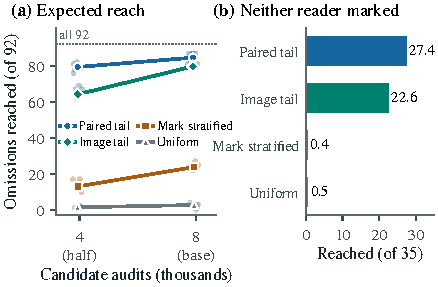
\includegraphics[width=\columnwidth]{acquisition}
\caption{\textbf{Audit reach.} (a)~Expected number of the 92 training omissions with at least one audited candidate (Eq.~\ref{eq:reach}), at the half and base budgets; faint points are the six matched draws. (b)~At half budget, expected reach among the 35 omissions on which neither weak reader placed a mark.}
\label{fig:acquisition}
\end{figure}

\begin{figure*}[t]
\centering
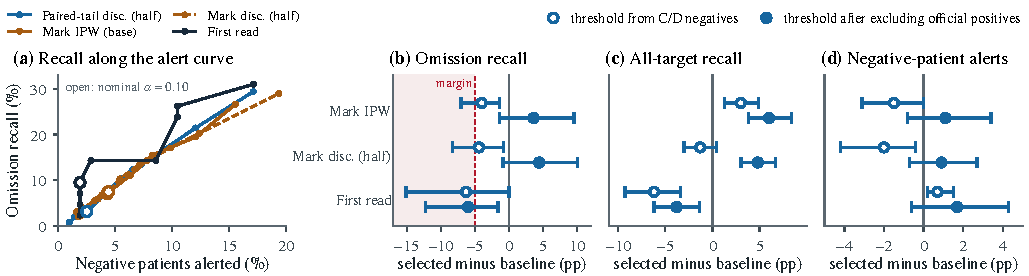
\includegraphics[width=\textwidth]{effects}
\caption{\textbf{Method comparison under two negative pools.} (a)~Mean omission recall against mean realized alerts over the calibration-derived cutoffs; open markers are the nominal $\alpha=0.10$ points of Tab.~\ref{tab:alloc}. (b--d)~Selected method minus each baseline, six-draw mean with 95\% patient-bootstrap intervals, using the same scores and the same 42 omissions, 276 targets and 90 common-negative test patients. Open circles: cutoff from C/D negatives; purple diamonds: cutoff after excluding patients with an official consensus nodule. The shaded region in (b) lies beyond the prespecified non-inferiority margin.}
\label{fig:effects}
\end{figure*}

On the 445 training patients, half-budget paired-tail sampling audits about 3,940 candidates and reaches \ReachPair{} of the 92 omissions in expectation (Fig.~\ref{fig:acquisition}a), whereas mark stratification at the base budget audits about 7,930 candidates and reaches \ReachMark{}. At the same half budget, image-tail sampling reaches \ReachImage{}, mark stratification 13.0 and uniform sampling 1.4. Most of the gain is therefore due to the image ranking, with the paired marks contributing a further 15.2 omissions on average and between 10 and 17 in each of the six matched draws. The realized draws are consistent with these expectations, ranging from 76 to 82 omissions for paired-tail sampling, 62 to 69 for image-tail sampling and 22 to 27 for base-budget mark stratification.

The improvement persists for the 35 omissions on which neither weak reader placed a mark, where the marks cannot point to the target directly (Fig.~\ref{fig:acquisition}b). Paired-tail sampling reaches 27.4 of them, compared with 22.6 for image-tail sampling and 0.4 for mark stratification at the same budget (0.9 at the base budget). In this case the marks act indirectly, by changing how the budget is distributed over the entire roster and thereby freeing reviews for highly ranked unmarked candidates. Since both paired-tail sampling and mark stratification touch nearly all 445 patients, the gain stems from which candidates are reviewed within each scan rather than from opening more scans.

\subsection{Effect of the representation}

With full reference labels, 3D features recover \OriginalLearned{} of the 276 test targets, compared with \OriginalDescriptor{} for the hand-crafted descriptors, a paired gain of 9.8 points [3.6, 16.6], while negative-patient alerts fall from 12 to 2 of 105. The fraction of covered targets that outrank every non-target candidate in their scan rises from 33.6\% to 67.9\%. As both heads share the same candidate locations, this comparison isolates the representation, and we use the 3D features in all remaining experiments.

\subsection{Main results}
\label{sec:locked}

\begin{figure*}[t]
\centering
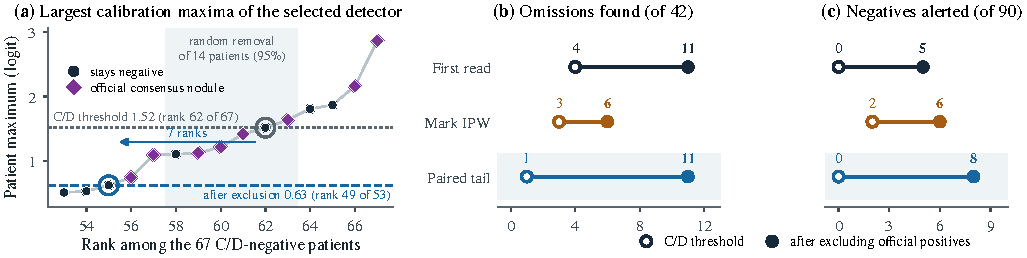
\includegraphics[width=\textwidth]{reference_tail}
\caption{\textbf{Threshold displacement at fixed scores.} (a)~The 15 largest maxima of the 67 C/D-negative calibration patients for the selected detector. Purple diamonds have a nodule in the official LUNA16 consensus. Excluding the 14 such patients moves the cutoff from rank 62 to the score at rank 55, while removing 14 patients at random puts it within the shaded ranks 58--63 (central 95\%). (b)~Omissions found among the same 42 targets, and (c)~alerts among the same 90 common-negative test patients, under the two cutoffs.}
\label{fig:tail}
\end{figure*}

\begin{table}[t]
\centering
\small
\setlength{\tabcolsep}{3.4pt}
\caption{\textbf{Locked results under the C/D reference} at nominal $\alpha=0.10$, mean of six matched draws. Omit.: recall on 42 test omissions (\%); All: recall on 276 targets (\%); Alert: negative patients alerted (\%). Half and base are audit budgets; disc.: discriminative augmentation (Eq.~\ref{eq:augmentation}). The selected method is in bold.}
\label{tab:alloc}
\begin{tabular}{lrrrr}
\toprule
Method & Omit.\,$\uparrow$ & All\,$\uparrow$ & Alert & FP/scan\,$\downarrow$ \\
\midrule
First read & \textbf{9.5} & \textbf{29.3} & 1.9 & 0.22 \\
nnPU (base) & 7.1 & 22.6 & 1.9 & 0.20 \\
Mark IPW (base) & 7.1 & 20.1 & 4.3 & 0.16 \\
Mark disc. (half) & 7.5 & 24.5 & 4.4 & 0.16 \\
Uniform disc. (half) & 7.9 & 24.9 & 5.9 & 0.16 \\
Image-tail disc. (half) & 4.8 & 23.2 & 2.4 & 0.17 \\
Paired-tail disc. (half)$^\dagger$ & 3.2 & 23.1 & 2.5 & 0.15 \\
Paired-tail IPW (half) & 4.0 & 24.9 & 2.5 & 0.15 \\
Paired-tail weighted (half) & 2.8 & 26.0 & 2.7 & \textbf{0.14} \\
\bottomrule
\end{tabular}

\end{table}

Table~\ref{tab:alloc} reports all training methods. Compared with base-budget mark IPW, the selected method uses \AuditSave\% fewer audits and raises all-target recall from 20.1\% to 23.1\%, a paired gain of 3.0 points [1.3, 4.9], at a lower alert rate (2.5\% vs.\ 4.3\%) and a similar FP/scan (0.15 vs.\ 0.16). On the primary endpoint, however, the selected method falls short. Its omission recall is \PairPrimary\%, against \IpwPrimary\% for mark IPW, a difference of $-4.0$ points [$-7.0$, $-1.4$] whose lower limit lies below the $-5$-point margin (Fig.~\ref{fig:effects}b, open circles). The conclusion is unchanged at matched alert rates: selecting each method's threshold on one calibration subset so that their alert rates on the other subset agree yields a difference of $-3.6$ points [$-7.0$, $-0.9$].

First-read training, which uses reader A's marks directly, achieves an omission recall of 9.5\%, and the half-budget mark, uniform and image-tail controls with the same estimator reach 7.5\%, 7.9\% and 4.8\%. Along the full alert curve (Fig.~\ref{fig:effects}a), first-read training leads below an alert rate of 3\%, while the audited methods remain close to one another at every rate. Results for a controlled setting in which the first reader keeps only its largest mark per scan, creating 151 imposed test omissions, are reported in the supplement.

\subsection{Analysis of missed omissions}
\label{sec:misses}

\begin{figure*}[t]
\centering
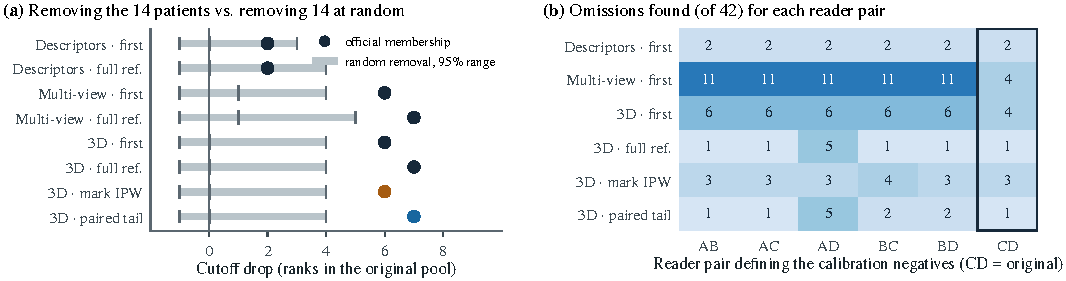
\includegraphics[width=\textwidth]{robustness}
\caption{\textbf{Robustness of the threshold displacement.} (a)~Cutoff drop on the original rank scale after excluding official-positive patients (dots), against the central 95\% range (bar, with median tick) of 8,192 subset-matched random removals. (b)~Omissions found among the same 42 targets after calibrating on the negatives of each reader pair; the boxed column is the original C/D reference.}
\label{fig:robust}
\end{figure*}

Every one of the 42 test omissions is covered by at least one candidate, so the roster itself is not the bottleneck. For the selected detector at the anchor draw, 16 omissions outrank every non-target candidate in their scan, yet only one of them exceeds the threshold. Of the 41 missed omissions, 26 are outranked by a non-target candidate in the same scan, whereas the remaining 15 win this within-scan comparison but stay below the threshold by a median of 2.22 logits. For the latter group, the failure occurs at the threshold rather than in the ranking.

The candidates that determine the threshold are unusual. Among the 45,541 candidates on C/D-negative calibration scans, only 74 lie near a contour drawn by just one of the reference readers C and D. Nevertheless, all three sampled maxima around the threshold carry this flag, as do both maxima that trigger alerts on C/D-negative test patients, and both of the latter match official LUNA16 targets. This concentration motivates the analysis of the negative pool in the next section.

\section{Effect of the Calibration Reference}
\label{sec:tail}

\subsection{Threshold displacement}

Excluding scans with an official consensus nodule removes 14 of the \PCal{} negative calibration patients and leaves \UCal{}. Three of the six largest maxima of the selected detector belong to excluded patients, and each of them matches an official nodule in 3D (Fig.~\ref{fig:tail}a). The original threshold is the 62nd score, a logit of \PairCutoffP{}, whereas the new threshold is the 49th of 53 scores, a logit of \PairCutoffU{} that ranked 55th in the original pool, a drop of \PairDrop{} ranks. Removing 14 patients at random, with the same number per calibration subset, moves the threshold by a median of \PairRobustMedian{} ranks and by at most \PairControlHi{} ranks in 95\% of the draws. The displacement is therefore driven by which patients are removed, not by the reduced pool size.

At the lower threshold, the same scores recover \PairHitsU{} of the 42 omissions instead of \PairHitsP{} (Fig.~\ref{fig:tail}b), and five of the ten additional detections were already ranked above every non-target candidate in their scan. Alerts on the same \UTest{} test patients increase from \PairAlertsP{} to \PairAlertsU{} (Fig.~\ref{fig:tail}c), which is consistent with the nominal rate of 10\%.

\subsection{Robustness}

We repeated the replay for all \NHeadRows{} fitted configurations, which yield \NHeads{} distinct score vectors over hand-crafted, multi-view and 3D features. The threshold falls for \LowerHeads{} of them, by a median of \MedianDrop{} ranks, and for \PastBand{} the drop exceeds the 95\% range of random removal. Since these score vectors share patients and include correlated training variants, the count indicates the breadth of the effect rather than independent replications.

Fig.~\ref{fig:robust}a and Tab.~\ref{tab:reference} detail eight representative detectors. The thresholds of the descriptor heads move by two ranks, within the random range, and both heads retain their two omission detections. In contrast, every learned head moves by six or seven ranks, outside the random range. A lower threshold produces additional detections only when the representation places targets between the two thresholds: the 3D first-read and full-reference heads gain 7 and 9 omissions, respectively, but the mark IPW head gains only 3. Changing the reader pair that defines the negatives yields between one and five detections for the selected detector, with at most one alert among the \RoleTest{} patients that are negative under every pair and under the official list (Fig.~\ref{fig:robust}b). The multi-view and 3D first-read heads detect 11 and 6 omissions, respectively, with every pair except the original C/D.

\begin{table}[t]
\centering\small
\setlength{\tabcolsep}{3pt}
\caption{\textbf{Fixed scores under two negative pools.} Each cell gives the count under the C/D cutoff $\to$ the count after excluding official-positive patients. Omit.: of 42 omissions; All: of 276 targets; Alert: of 90 common-negative test patients. Drop: cutoff drop in ranks of the original pool.}
\label{tab:reference}
\begin{tabular}{lrrrr}
\toprule
Scorer / training & Omit. & All & Alert & Drop \\
\midrule
Descriptors / first & 2 $\to$ 2 & 39 $\to$ 55 & 7 $\to$ 12 & 2 \\
Descriptors / full ref. & 2 $\to$ 2 & 47 $\to$ 57 & 7 $\to$ 10 & 2 \\
Multi-view / first & 4 $\to$ 11 & 66 $\to$ 125 & 1 $\to$ 7 & 6 \\
Multi-view / full ref. & 3 $\to$ 11 & 69 $\to$ 142 & 1 $\to$ 9 & 7 \\
3D / first & 4 $\to$ 11 & 81 $\to$ 133 & 0 $\to$ 5 & 6 \\
3D / full ref. & 1 $\to$ 10 & 74 $\to$ 140 & 0 $\to$ 8 & 7 \\
3D / mark IPW & 3 $\to$ 6 & 70 $\to$ 91 & 2 $\to$ 6 & 6 \\
3D / paired tail & 1 $\to$ 11 & 69 $\to$ 138 & 0 $\to$ 8 & 7 \\
\bottomrule
\end{tabular}

\end{table}

\subsection{Effect on the method comparison}

Averaged over the six matched draws, excluding official positives raises the omission recall of the selected method by \PairChange{} points \PairChangeCI{}. Its difference to mark IPW moves from $\PairRelativeP$ to $+\PairRelativeU$ points \PairRelativeUCI{}, a shift of \ReferenceInteraction{} points \ReferenceInteractionCI{} (Fig.~\ref{fig:effects}b). The same reversal occurs against mark stratification with the same estimator ($-4.4$ to $+4.4$ points), whereas the gap to first-read training remains negative. The gains in all-target recall increase under the new pool (Fig.~\ref{fig:effects}c), and the alert differences stay within about two points (Fig.~\ref{fig:effects}d), with realized alert rates of 7.2\% for paired-tail sampling and 6.1\% for mark IPW. The primary conclusion of Sec.~\ref{sec:locked} thus hinges on how the negative pool is defined rather than on the scores themselves.

\begin{figure}[t]
\centering
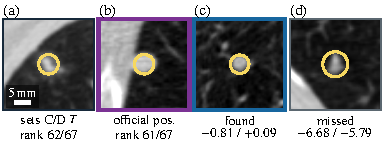
\includegraphics[width=\columnwidth]{ct_evidence}
\caption{\textbf{CT examples} (axial, 28\,mm field of view; circle: matching radius). (a)~The candidate that sets the C/D cutoff. (b)~A neighbouring calibration maximum on a scan with an official consensus nodule (purple frame). (c)~A test omission found only under the lower cutoff (blue frame). (d)~An omission below both cutoffs, outscored by a non-target candidate in its scan. Margins: best target logit minus the C/D and the new cutoff.}
\label{fig:ct}
\end{figure}

\paragraph{Qualitative examples.}
Fig.~\ref{fig:ct} relates these ranks to images. A consensus-positive maximum, shown in (b), leaves the negative pool with its score unchanged. A test omission, shown in (c), then exceeds the lower threshold with the same image, location and score. Other omissions, such as (d), remain far below both thresholds, which illustrates why ranking and calibration need to be assessed separately.


\section{Discussion and Limitations}
\label{sec:discussion}

\paragraph{Reach is not detection.}
Paired-tail sampling places reviews where omissions are, so it reveals many more of them. The detector trained on these labels is still a linear head on a frozen embedding, and at the locked cutoff almost no omission crosses the threshold for any training method (Sec.~\ref{sec:misses}). Better labels therefore move scores, but rarely past the cutoff. Whether a stronger, end-to-end learner turns the extra reach into extra detections is open.

\paragraph{Reference membership is part of the operating point.}
At a 10\% patient alert rate with 67 calibration negatives, the cutoff is the sixth-largest maximum, so a handful of patients decide it. We recommend reporting the reference status of the maxima near the cutoff, replaying the scores under an alternative negative pool, and comparing target recovery and alerts on common test support, as in Sec.~\ref{sec:tail}.

\paragraph{Limitations.}
The audit benefit is counted in candidate decisions. Both mark-based policies touch almost every training patient, and reading time, the cost of an extra read and the cost of selecting candidates are not measured. The candidate roster inherits the LUNA16 proposal sources, some developed on the same LIDC scans. All references reuse the same unblinded LIDC reader records, and no independent adjudication decides whether the disputed maxima are in-scope nodules. LUNA16 is public and has been studied extensively, so our evaluation is retrospective even though all weights, endpoints and contrasts were frozen before the calibration and test subsets were scored. The reference replay was specified after the locked comparison and is reported as a follow-up. Replication on new patients with independent adjudication would test how far the calibration effect transfers. This secondary analysis uses released, de-identified images and annotations, with no participant interaction or new data collection.

\section{Conclusion}
\label{sec:conclusion}

We separated what an audit reveals from what a detector recovers and from where its alert threshold falls. A probability audit guided by scan rank and reader disagreement finds far more unmarked nodules per review than mark-stratified review. Those labels did not raise omission recall at the locked threshold. The threshold itself moved by several ranks when only 14 consensus-positive patients left the negative pool, with all scores fixed, and the method comparison changed sign. Low-alert evaluations of lesion detectors should treat the negative reference as a modelling decision and report its effect.
\fi

\begin{samepage}
\section*{LLM Usage Statement}
OpenAI Codex assisted with experimental design, analysis code and execution, data-derived figure preparation, literature checks, and drafting and editing the manuscript and supplement. Claude (Anthropic) assisted with revising the text, redrawing the figures from the reported values, and checking references. The authors take full responsibility for the content.
\end{samepage}

{\small
\bibliographystyle{ieeenat_fullname}
\bibliography{references}
}
\end{document}
